
%(BEGIN_QUESTION)
% Copyright 2006, Tony R. Kuphaldt, released under the Creative Commons Attribution License (v 1.0)
% This means you may do almost anything with this work of mine, so long as you give me proper credit

Beregn verdier i følgende kalibreringstabell for en deplacement-basert nivåtransmitter som måler væskenivågrensesnitt (tettheter = 50 lb/ft$^{3}$ og 70 lb/ft$^{3}$), med kalibreringstoleranse $\pm$ 1\%:

$$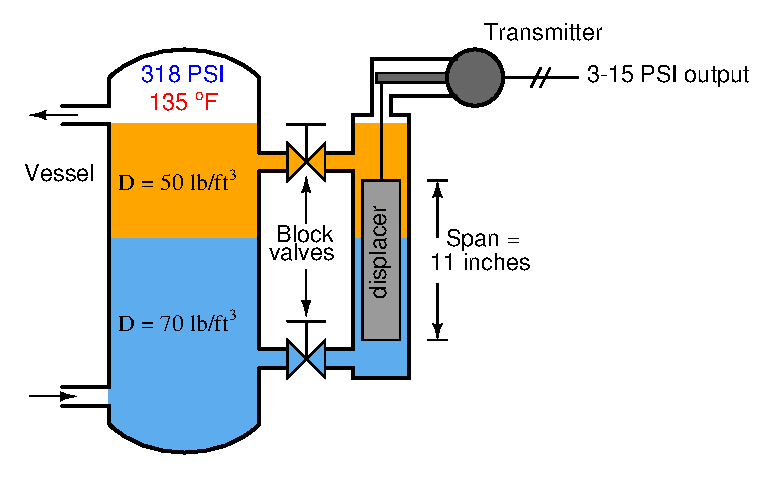
\includegraphics[width=15.5cm]{i00687x01.eps}$$

% No blank lines allowed between lines of an \halign structure!
% I use comments (%) instead, so that TeX doesn't choke.

$$\vbox{\offinterlineskip
\halign{\strut
\vrule \quad\hfil # \ \hfil &
\vrule \quad\hfil # \ \hfil &
\vrule \quad\hfil # \ \hfil &
\vrule \quad\hfil # \ \hfil &
\vrule \quad\hfil # \ \hfil &
\vrule \quad\hfil # \ \hfil \vrule \cr
\noalign{\hrule}
%
% First row
Grensesnitt- & Prosent av & Oppdrifts- & Utgangssignal & Utgangssignal & Utgangssignal \cr
%
% Another row
nivå (in) & span (\%) & kraft (lbs) & ideal (PSI) & min. (PSI) & max. (PSI) \cr
%
\noalign{\hrule}
%
% Another row
  & 0 &  &  &  &  \cr
%
\noalign{\hrule}
%
% Another row
  & 10 &  &  &  &  \cr
%
\noalign{\hrule}
%
% Another row
  & 25 &  &  &  &  \cr
%
\noalign{\hrule}
%
% Another row
  & 50 &  &  &  &  \cr
%
\noalign{\hrule}
%
% Another row
  & 75 &  &  &  &  \cr
%
\noalign{\hrule}
%
% Another row
  & 90 &  &  &  &  \cr
%
\noalign{\hrule}
%
% Another row
  & 100 &  &  &  &  \cr
%
\noalign{\hrule}
} % End of \halign
}$$ % End of \vbox

Anta følgende deplacementdata:

\begin{itemize}
\item{} Form: {\it sylindrisk}
\item{} Lengde = 11 inches
\item{} Diameter = 1.5 inches
\item{} Tørrvekt = 2.7 lbs
\end{itemize}

\vskip 10pt

Vis hele utregningen slik at instruktøren kan verifisere framgangsmåten din.

\vskip 20pt \vbox{\hrule \hbox{\strut \vrule{} {\bf Forslag til sokratisk diskusjon} \vrule} \hrule}

\begin{itemize}
\item{} Hvordan responderer transmitteren hvis gasstrykket i beholderen øker?
\item{} Hvordan responderer transmitteren hvis gasstrykket i beholderen synker?
\item{} Hvordan responderer transmitteren hvis totalt væskenivå synker under toppen av deplacementelementet?
\item{} Har det betydning for kalibreringen om deplacementelementet er massivt eller hult?
\item{} Vis hvordan man kan {\it estimere} numeriske svar uten kalkulator.
\end{itemize}

\underbar{file i00687no}
%(END_QUESTION)





%(BEGIN_ANSWER)

\noindent
{\bf Delvis svar:}

% No blank lines allowed between lines of an \halign structure!
% I use comments (%) instead, so that TeX doesn't choke.

$$\vbox{\offinterlineskip
\halign{\strut
\vrule \quad\hfil # \ \hfil &
\vrule \quad\hfil # \ \hfil &
\vrule \quad\hfil # \ \hfil &
\vrule \quad\hfil # \ \hfil &
\vrule \quad\hfil # \ \hfil &
\vrule \quad\hfil # \ \hfil \vrule \cr
\noalign{\hrule}
%
% First row
Grensesnitt- & Prosent av & Oppdrifts- & Utgangssignal & Utgangssignal & Utgangssignal \cr
%
% Another row
nivå (in) & span (\%) & kraft (lbs) & ideal (PSI) & min. (PSI) & max. (PSI) \cr
%
\noalign{\hrule}
%
% Another row
0 & 0 & 0.5625 & 3 & 2.88 & 3.12 \cr
%
\noalign{\hrule}
%
% Another row
1.1 & 10 & 0.5850 & 4.2 & 4.08 & 4.32 \cr
%
\noalign{\hrule}
%
% Another row
2.75 & 25 & 0.6187 & 6 & 5.88 & 6.12 \cr
%
\noalign{\hrule}
%
% Another row
5.5 & 50 & 0.6750 & 9 & 8.88 & 9.12 \cr
%
\noalign{\hrule}
%
% Another row
8.25 & 75 & 0.7312 & 12 & 11.88 & 12.12 \cr
%
\noalign{\hrule}
%
% Another row
9.9 & 90 & 0.7649 & 13.8 & 13.68 & 13.92 \cr
%
\noalign{\hrule}
%
% Another row
11 & 100 & 0.7874 & 15 & 14.88 & 15.12 \cr
%
\noalign{\hrule}
} % End of \halign
}$$ % End of \vbox

%(END_ANSWER)





%(BEGIN_NOTES)

Her er de to "tankeeksperiment"-scenarioene som brukes for å finne LRV- og URV-trykkverdier:

$$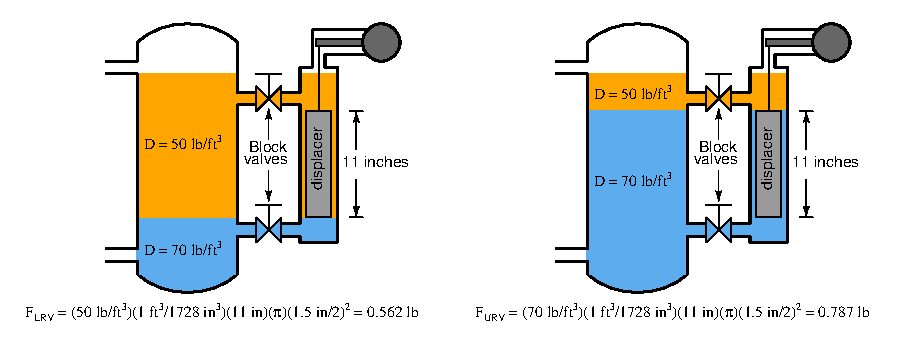
\includegraphics[width=15.5cm]{i00687x02.eps}$$

\vskip 10pt

Vapor-space dataene (318 PSI og 135 $^{o}$F) er overflødig informasjon, med hensikt lagt inn for å teste om studenten kan avgjøre hva som er relevant i problemet.

%INDEX% Måling, grensesnittnivå: deplacement (oppdrift)

%(END_NOTES)
